\section{Architecure}
The “4+1 view model”\footnote{Kruchten, Philippe (1995, November). Architectural Blueprints — The “4+1” View Model of Software Architecture. IEEE Software 12 (6), pp. 42-50.} by Philippe Kruchten suggest four different view, logical, process, development and physical. In the case of XOXOMail we are going to use the logical, process and development view. The rationale behind removing the physical view is that XOXOMail will run on a single physical device and only utilize one process, a security view, describing how the layers of security is implemented around and in the application.

\subsection{Logical view (Object oriented deomposition)}
“The logical architecture primarily supports the functional requirements --- what the system should provide in terms of services to its users. The system is decomposed into a set of key abstractions, taken from the problem domain, in the form of objects or object classes” \footnote{Kruchten, Philippe (1995, November). Architectural Blueprints — The “4+1” View Model of Software Architecture. IEEE Software 12 (6), pp. 42-50.} A common way to represent this is view is with a class diagram that shows a set of classes and their relationships.

\begin{figure}
	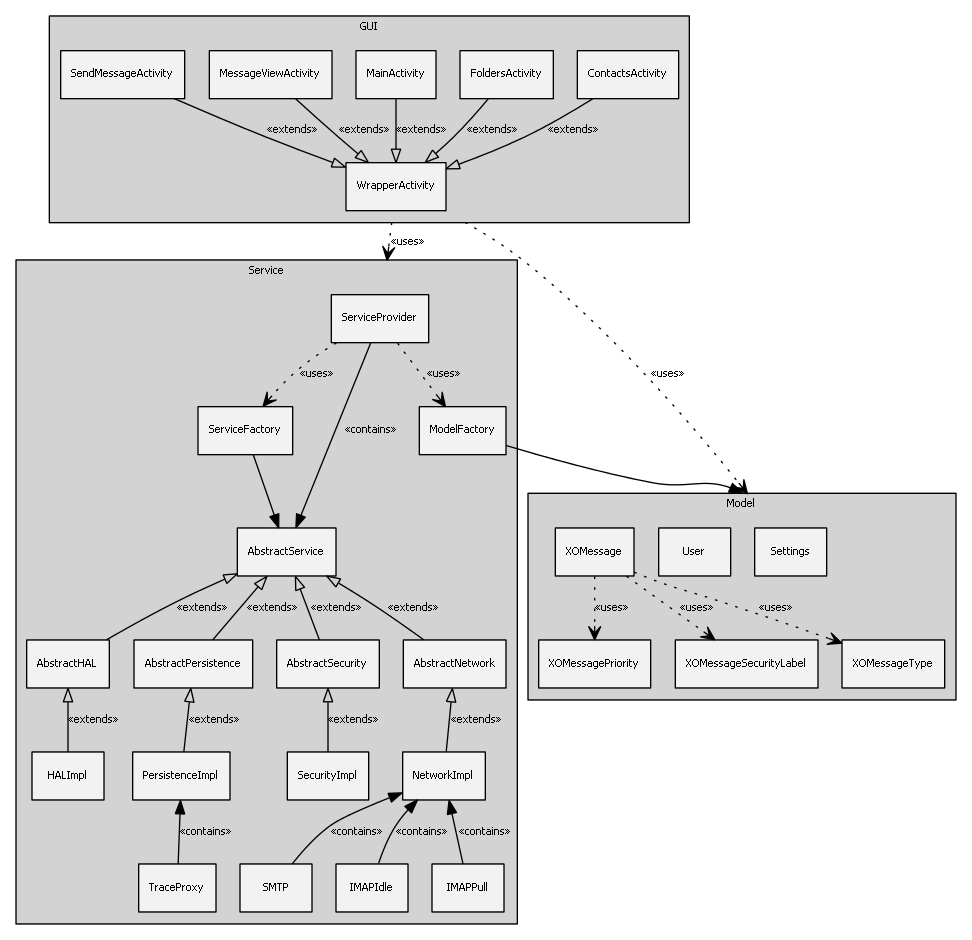
\includegraphics[width=\textwidth]{logicalview.png}
	\caption{The logical view of the architecture}
	\label{fig:logicalview}
\end{figure}

\subsection{Development view (Subsystem decomposition)}
The development view is a step up from the logical view and focuses on software modules instead of classes. These subsystems/modules are organized in a hierarchy of layers where each layer provides a well-defined interface to layers above. “The complete development architecture can only be described when all the elements of the software have been identified. It is, however, possible to list the rules that govern the development architecture: partitioning, grouping, visibility.“
\subsection{Process View}
\subsection{Security View}

\subsection{GUI}
\begin{figure}
	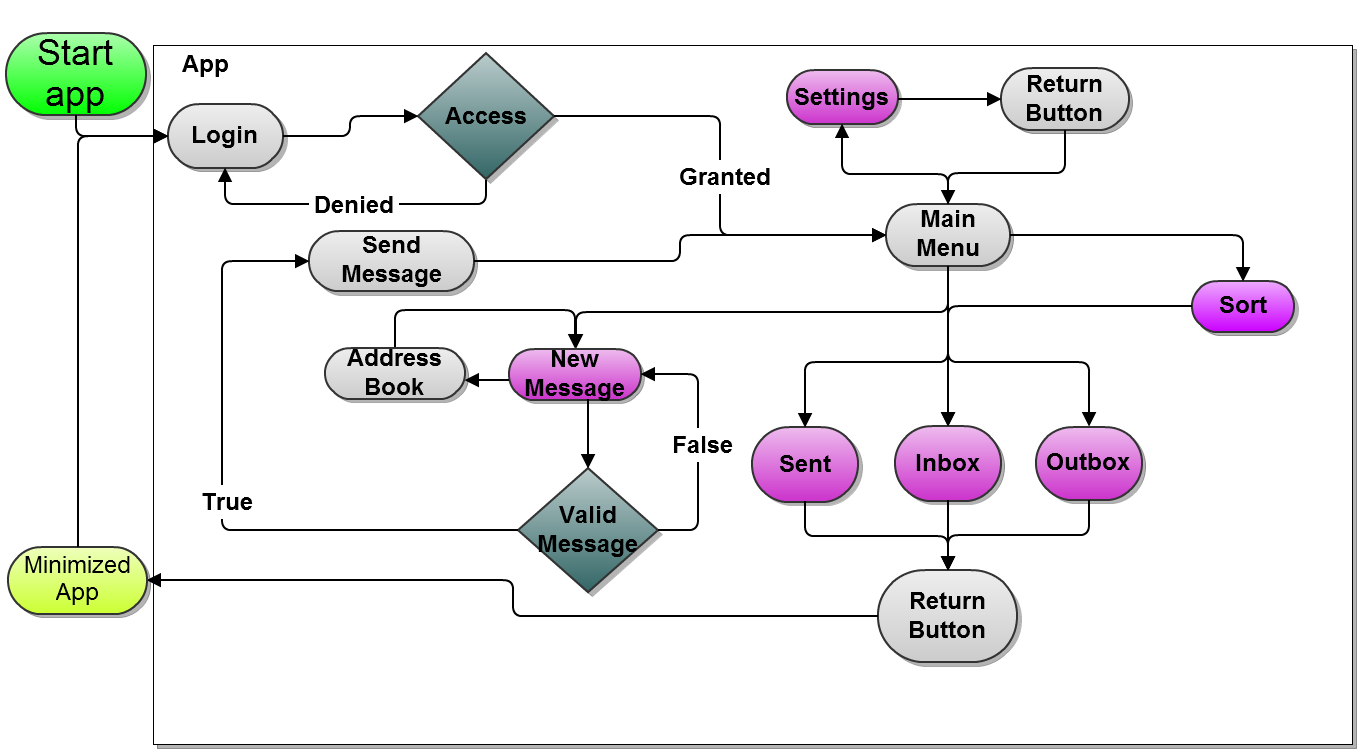
\includegraphics[width=\textwidth]{Android_GUI_flow_chart_2}
	\caption{The logical view of the GUI architecture}
	\label{fig:logicalGUIview}
\end{figure}